\section{The Visualization Composition Model}
\label{sec:model}
Designing a visualization for a particular dataset from scratch is an extremely complicated process.  To accomplish this task, the designer needs to first choose or craft a visual representation that is suitable for the data and then map the data onto the graphical primitives that the visual form will be composed of.  These choices, mappings and compositions can be thought of as a visualization composition process.  In VisComposer, we define this  process as a model consisting of the following modules:

The \textbf{Resource} module consists of four classes of information: the underlying data, a set of basic primitives, a set of composition operators and a list of visual forms. The \emph{input dataset} is represented with a specified format which contains the data and extra information that defines the data types. The \emph{primitives} denote the basic graphical presentations for constructing a visualization. They can be evaluated and rendered with respect to different platforms. For instance, our implementation employs the basic SVG primitives introduced in HTML5.
 Each primitive contains a name, a set of visual properties, and links to the bound data. Each \emph{composition operator} defines the layout and organization of the primitives. A \emph{visual form} refers to a design template that consists of a group of primitives and their compositions. The visual forms can be created, stored, and altered for fast prototyping and sharing.

The \textbf{Visualization} module denotes the result of applying a visualization pipeline or a visual form (template) to an input dataset. In principle, a visualization is composed of graphical primitives by means of the composition operators. Thus, composing the primitives with the assistance of the composition operators is the basic task in designing a visualization. 
%\textit{Taking the creation of scatter-plot as an example, once a scenegraph is finished, in the visualization module the pipeline will be applied to a dataset, and the points derived will be rendered in a coordinate system.}
%%the visual forms and coordinates of each point is derived from the input dataset by applying the

The \textbf{Scenegraph} module is a structural abstraction of a visualization. It employs a tree structure to encode how the primitives are organized in the drawn view. We employ the tree organization to allow for composition of multiple visual representations in a visualization. Each node of a tree is bound to selected data items and primitives while each link represents the data transformations and primitives arrangement of linked nodes. Nodes and links are created using primitives and composition operators of the \textbf{Resource} module, respectively. They are editable and programmable.

The \textbf{Transformation} module denotes a workspace that accommodates three types of user-controllable operations: filtering data, specifying the visual properties of primitives, and binding selected data items, primitives and composition operators to corresponding elements of a scenegraph.

%The underlying dataset can be processed and distributed from the root node to leaf nodes of the scenegraph.   To support the distribution and transfer of data items, related data items can either undergo visualization operations, or be distributed into other nodes in the scenegraph. If visualization operations are chosen, each node is expanded to several instances, of which the number depends on the bound data.  The data flow is iterated, yielding a nested tree structure, as shown in Fig.~\ref{fg:pipeline_2}.

    Figure~\ref{fg:model} (a) illustrates the relationships among the four modules. After a dataset is loaded, it is filtered, enumerated or selected into many groups of data items. In the meantime, the set of primitives can be selected and arbitrarily combined with the composition operators. The entire composition process includes two parts. The first part specifies or modulates the organization of the intended visualization within the \textbf{Scenegraph}, and the second part transforms, binds, and specifies the visual mapping of the scenegraph elements within the \textbf{Transformation}.

The proposed composition model is different from the ones used in iVisDesigner~\cite{Yuan:2014:TVCG} or Lyra~\cite{Heer:2014:CGF} which allow the user to directly manipulate the graphical elements in the visualization canvas.  Our model allows for both the manipulation of elements on a canvas while providing an additional design space through the Scenegraph and Transformation modules. While the direct manipulation mode enables dynamic design and facilitates a What You See Is What You Get visual editor, it is inefficient to design complicated visual forms (e.g., recursive drawings) or specify visual styles for massive individual visual elements (e.g., specifying colors of 1000 primitives based on a certain criteria). Our model explicitly employs an editable abstraction to the visualization thereby enabling a flexible customization of special visualization effects and eliminates the workload of manual specification of visual designs with selected programmability.

We illustrate our model by creating a sample visualization of a 4D dataset containing 150 points (see Figure~\ref{fg:interface}).  In this example, we have chosen a scatterplot matrix to be the visual form. The Resource module inputs the dataset and passes the dimension number (i.e., 4) to the Scenegraph module. Two types of primitives (point and axis) and the composition operators (uniform subdivision) are selected for composing the visualization in the Scenegraph and Transformation modules. In particular, the Scenegraph module generates a 3-level tree: the root node represents the entire visualization, the middle level nodes encode $4\times4 =16 $ matrix cells, and the leaf nodes correspond to $4 \times 4 \times 150$ primitives. The links of the Scenegraph encode the 3-level embedding structure of the scatterplot matrix, and determine the layout, composition and coordinate systems of the visualization. The Transformation module binds the nodes and edges of the Scenegraph to selected and filtered data, and specifies the visual properties of the primitives.

\begin{figure}
  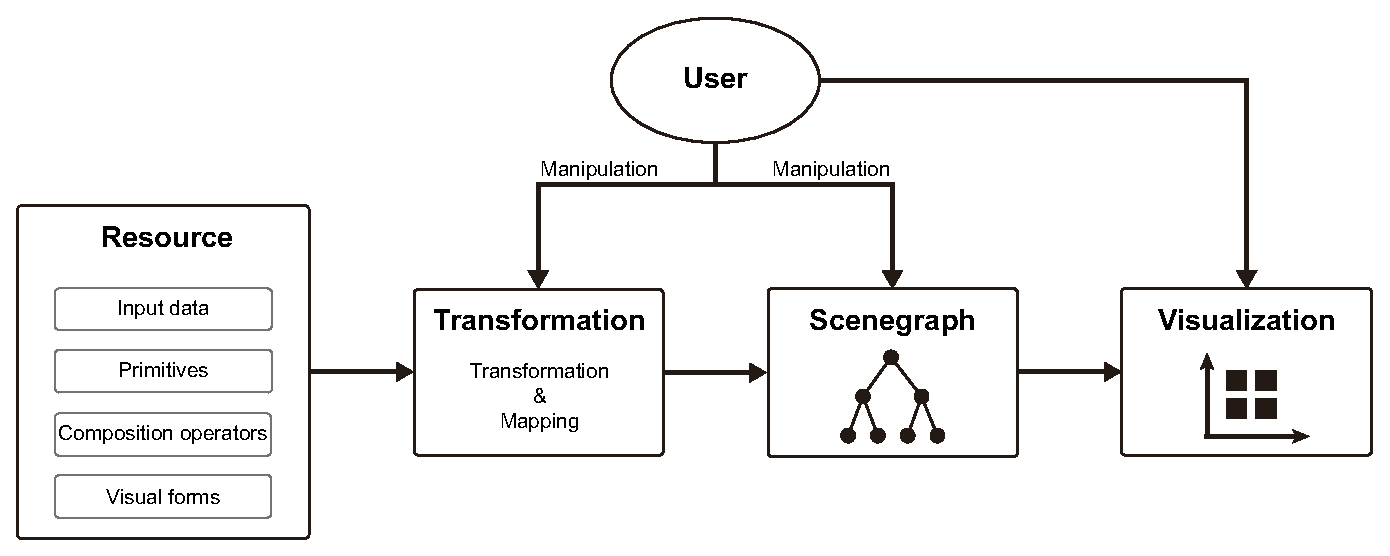
\includegraphics[width=0.98\linewidth]{images/compositionModel.eps}
  \caption{The visualization composition model consists of four modules.} \label{fg:model}
\end{figure}
